\documentclass[aspectratio=169]{beamer}
\usetheme{Informatics}

\usepackage[backend=biber, style=ieee, maxcitenames=6]{biblatex}
\addbibresource{bib.bib}
\usepackage{csquotes}

\usepackage{tikz}
\usepackage{tikz-3dplot}
\usepackage{tikzpeople}
\usetikzlibrary{arrows, arrows.meta, fadings, fit, backgrounds, calc, math, decorations.markings, decorations.text, intersections, patterns, bending, positioning, shapes, shapes.geometric}
% set up externalization
\usetikzlibrary{external}
\tikzexternalize[
  prefix=Tikz/,
  ]
\tikzset{%
  external/only named=true,
  block/.style = {draw, rounded corners=2ex, outer sep=0, minimum width=2.2cm, fill=white},%
  masterBlock/.style = {fill, rectangle, inner sep=0.1*\U, rounded corners=2ex, fill=infoBlue!20!white},
  frame/.style={rectangle, draw, minimum width=5em, text centered, minimum height=3.6em, fill=white, rounded corners, align=center},
  line/.style={draw, -{Latex}},
}
\usepackage{pgfplots}
\usepackage{pgfplotstable}
\pgfplotsset{compat=newest}
\pgfplotsset{%
  % grid=both,
  tick align=outside,
  tick pos=left,
  major tick length=2pt,
  xlabel shift = -3 pt,
  ylabel shift = -3 pt,
  % enlargelimits=false,
  every axis plot/.append style={%
      font=\footnotesize,
  }, % line
  legend cell align={left},
  every axis legend/.append style={%
      font=\footnotesize,
  },
  every tick label/.append style={%
      font=\footnotesize,
  },
}
\usepackage{countriesofeurope}
\usepackage{fontawesome}
\usepackage{subcaption}
\makeatletter
\newcommand{\getLength}[4]{%
    \pgfmathanglebetweenpoints{\pgfpointanchor{#1}{#2}}
                              {\pgfpointanchor{#3}{#4}}
    \global\let\myangle\pgfmathresult % we need a global macro
    \pgfpointdiff{\pgfpointanchor{#1}{#2}}
                {\pgfpointanchor{#3}{#4}}
    \pgf@xa=\pgf@x % no need to use a new dimen
    \pgf@ya=\pgf@y
    \pgfmathparse{veclen(\pgf@xa,\pgf@ya)/28.45274} % to convert from pt to cm
    \global\let\mylength\pgfmathresult % we need a global macro
}
\makeatother 

\usepackage{siunitx}
\usepackage{bm}
\usepackage{xcolor}
\colorlet{myorange}{orange!80!black}
\colorlet{myred}{red!80!black}
\colorlet{myblue}{blue!80!black}
\colorlet{mygreen}{green!60!black}
\colorlet{mydarkred}{red!30!black}
\colorlet{mydarkblue}{blue!40!black}
\colorlet{mydarkgreen}{green!30!black}
\usepackage{listofitems} % for \readlist

\usepackage{wrapfig}
\usepackage{multirow}
\usepackage{multicol}
\usepackage{makecell}
\usepackage{qrcode}
\usepackage{hyperref}
\usepackage{multimedia}
\newcommand{\heightVideo}{6.0cm}
\newcommand{\heightVideoFull}{7.0cm}

\newrobustcmd*{\footfullcitenomark}{% 
  \AtNextCite{%
    \let\thefootnote\relax
    \let\mkbibfootnote\mkbibfootnotetext
  }
  \footfullcite%
}
\title{Deploying multi-contact manipulation}
\subtitle{Towards achieving dyynamic contact-rich manipulation behaviours}
\author{\textbf{Jo\~{a}o Moura}}
\date{\today}


\makeatletter
\def\calcLength(#1,#2)#3{%
\pgfpointdiff{\pgfpointanchor{#1}{center}}%
             {\pgfpointanchor{#2}{center}}%
\pgf@xa=\pgf@x%
\pgf@ya=\pgf@y%
\FPeval\@temp@a{\pgfmath@tonumber{\pgf@xa}}%
\FPeval\@temp@b{\pgfmath@tonumber{\pgf@ya}}%
\FPeval\@temp@sum{(\@temp@a*\@temp@a+\@temp@b*\@temp@b)}%
\FProot{\FPMathLen}{\@temp@sum}{2}%
\FPround\FPMathLen\FPMathLen5\relax
\global\expandafter\edef\csname #3\endcsname{\FPMathLen}
}
\makeatother

\begin{document}

\newsavebox{\nodeRL}
\savebox{\nodeRL}{%
    \tikzexternaldisable
    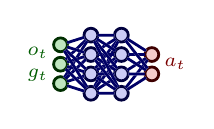
\begin{tikzpicture}[font=\scriptsize, x=1.1em, y=0.7em, inner sep=0.]
        % Definition of styles
        \tikzstyle{node}=[circle,draw=myblue,minimum size=0.5em,inner sep=0.0,outer sep=0.0]
        \tikzstyle{node in}=[node,green!20!black,draw=mygreen!30!black,fill=mygreen!25]
        \tikzstyle{node hidden}=[node,blue!20!black,draw=myblue!30!black,fill=myblue!20]
        \tikzstyle{node out}=[node,red!20!black,draw=myred!30!black,fill=myred!20]
        \tikzstyle{connect}=[mydarkblue] %,line cap=round
        \tikzset{ % node styles, numbered for easy mapping with \nstyle
            node 1/.style={node in},
            node 2/.style={node hidden},
            node 3/.style={node out},
        }
        \def\nstyle{int(\lay<\Nnodlen?min(2,\lay):3)} % map layer number onto 1, 2, or 3
        \coordinate (origin) at (0,0);
        % Constants for scalling
        \begin{scope}[transparency group]
            %----------------------------------------------------------------------------
            \readlist\Nnod{3,4,4,2} % array of number of nodes per layer
            \foreachitem \N \in \Nnod{ % loop over layers
            \def\lay{\Ncnt} % alias of index of current layer
            \pgfmathsetmacro\prev{int(\Ncnt-1)} % number of previous layer
            \foreach \i [evaluate={\y=\N/2-\i; \x=\lay; \n=\nstyle;}] in {1,...,\N}{ % loop over nodes
                % NODES
                \node[node \n] (N\lay-\i) at ($(origin)+(\x,\y)$) {};
                % CONNECTIONS
                \ifnum\lay>1 % connect to previous layer
                \foreach \j in {1,...,\Nnod[\prev]}{ % loop over nodes in previous layer
                    \draw[connect,white] (N\prev-\j) -- (N\lay-\i);
                    \draw[connect] (N\prev-\j) -- (N\lay-\i);
                }
                \fi % else: nothing to connect first layer
            }
            }
            % LABELS
            \node[left=0.4,align=center,mygreen!60!black] at (N1-2) {$o_t$\\$g_t$};
            \node[right=0.4,align=center,myred!60!black] at ($(N\Nnodlen-1)!0.5!(N\Nnodlen-2)$) {$a_t$};
            % \node[above=0.5,align=center,myblue!60!black] at ($(N2-1)!0.5!(N3-1)$) {$u=\pi(x)$};
            % \node[below=0.5,align=center,myblue!60!black] at ($(N2-\Nnodlen)!0.5!(N3-\Nnodlen)$) {$u=\pi(x)$};
            % \node[below=0.5,align=center] at ($(N2-\Nnodlen)!0.5!(N3-\Nnodlen)$) {\textbf{L}earning};
            %----------------------------------------------------------------------------
        \end{scope}
    \end{tikzpicture}%
    \tikzexternalenable
}

% figure pushing
\newsavebox{\nodePushing}%
\savebox{\nodePushing}{%
    \tikzexternaldisable
    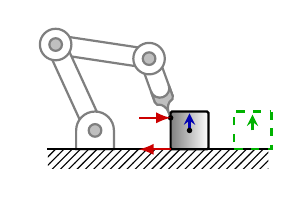
\begin{tikzpicture}
        % Definition of styles
        % function to compute angle and length between coordinates
\makeatletter
\newcommand{\getLengthAndAngle}[2]{%
    \pgfmathanglebetweenpoints{\pgfpointanchor{#1}{center}}
                              {\pgfpointanchor{#2}{center}}
    \global\let\myangle\pgfmathresult % we need a global macro
    \pgfpointdiff{\pgfpointanchor{#1}{center}}
                 {\pgfpointanchor{#2}{center}}
    \pgf@xa=\pgf@x % no need to use a new dimen
    \pgf@ya=\pgf@y
    \pgfmathparse{veclen(\pgf@xa,\pgf@ya)/28.45274} % to convert from pt to cm
    \global\let\mylength\pgfmathresult % we need a global macro
}
\makeatother 
\tikzset{
    pics/pivot/.style args={#1,#2,#3}{
		code = {
			% #1: radius of small circle (pin);
			% #2: radius of large circle (outer dimension).
            % #3: rotation angle
			\draw[thick, fill=white, rotate=#3] (#2,-#2) -- (#2,0) arc(0:180:#2) -- (-#2,-#2) -- cycle;
			\draw[thick, fill=gray] (0,0) circle circle (#1);
		}
	},
	ground/.style = {fill,pattern=north east lines,draw=none,minimum width=1cm,minimum height=1cm},
    spring/.style = {thick,decorate,decoration={zigzag,pre length=4pt,post length=4pt,segment length=3pt}},
    damper/.style = {thick, decoration={markings, mark connection node=dmp, mark=at position 0.5 with
              {
                \node (dmp) [thick,inner sep=0pt,transform shape,rotate=-90,minimum width=8pt,minimum height=2pt,draw=none] {};
                \draw [thick] ($(dmp.north east)+(2pt,0)$) -- (dmp.south east) -- (dmp.south west) -- ($(dmp.north west)+(2pt,0)$);
                \draw [thick] ($(dmp.north)+(0,-3pt)$) -- ($(dmp.north)+(0,3pt)$);
              }
        }, decorate},
	pics/dimLinear/.style args={#1,#2,#3,#4,#5,#6,#7}{
		code = {
			% #1: node 1
			% #2: node 2
			% #3: node 1 guide line distance
			% #4: node 2 guide line distance
			% #5: label distance
			% #6: label
			% #7: label position (ex: right, left, above, below)
			\draw[very thin, gray] ($(#1)!#3!-90:(#2)$) -- ($(#1)!#5+3pt!-90:(#2)$); % lateral line perpendicular to nodes 1 and 2
			\draw[very thin, gray] ($(#2)!#4!90:(#1)$) -- ($(#2)!#5+3pt!90:(#1)$); % lateral line perpendicular to nodes 1 and 2
			\draw[very thin, arrows=<->, gray] ($(#1)!#5!-90:(#2)$) -- ($(#2)!#5!90:(#1)$) node[midway, #7] {#6}; % dimension line parallel to nodes 1 and 2
		}
	},
	pics/dimAngular/.style args={#1,#2,#3,#4,#5,#6,#7,#8}{
		code = {
			% #1: node 1 (this node will define the distance the arc from the central node)
			% #2: node 2
			% #3: node centre
			% #4: distance before arrow ends
			% #5: node 1 guide line distance
			% #6: label
			% #7: label position (ex: right, left, above, below)
			% Create lines for computing arc centre
			\def\argone{#4}\def\argtwo{0}
			\ifx\argone\argtwo % if the arrow offset is zero the rotation centre remains the same
				\coordinate (centre) at (#3);
			\else % if there is offset we find the:
				\draw[name path=AB,draw=none] ($(#2)!#4!90:(#3)$) -- ($(#3)!#4!-90:(#2)$); % line parallel to the link formed by the nodes 1 and 2 with offset #4
				\draw[name path=CD,draw=none] (#1) -- (#3); % reference line for measure the angle
				\coordinate [name intersections={of={AB and CD}}]; % intersection between the offset line and the reference line
				\coordinate (centre) at (intersection-1); % set the rotation centre as the found intersection
			\fi
			\draw [very thin, gray, #8] let
				\p0 = ($(#1)-(centre)$), % difference vector between reference and centre
				\p1 = ($($(#2)!#4!90:(#3)$)-(centre)$) % difference vector reference between the offset line and the centre
				in (#1) arc [start angle={atan2(\y0,\x0)}, end angle={atan2(\y1,\x1)}, radius=({veclen(\y0,\x0)})] node[midway, #7] {#6}; % angular dimension line
			\draw[very thin, gray] ($(#3)!#5!0:(#1)$) -- ($(#1)!-3pt!0:(#3)$); % Draw guide line
		}
	},
    pics/link/.style args={#1,#2,#3}{
		code = {
			% #1: node 1
			% #2: node 2
			% #3: characteristic dimension of drawing
            \draw[thick, fill=white] ($(#1)!1.5*#3!-90:(#2)$) -- ($(#2)!1.5*#3!90:(#1)$) -- ($(#2)!1.5*#3!-90:(#1)$) -- ($(#1)!1.5*#3!90:(#2)$) -- cycle; % lines parallel to nodes 1 and 2
            \fill[white, draw=none] (#2) circle circle (2.5*#3); % outer round part
            \draw[thick] (#2) circle circle (2.5*#3); % outer round part
            \fill[gray, draw=none] (#2) circle circle (#3);
            \draw[thick] (#2) circle circle (#3);
		}
	},
	pics/centreofmass/.style args={#1,#2}{
		code = {
			% #1: radius of symbol
			\draw[fill=black, thin] (#2) -- ++(#1,0) arc [radius=#1, start angle=0,end angle=90] -- ++(0,-2*#1) arc [radius=#1, start angle=270, end angle=180] -- cycle;
			\draw[thin] (#2) circle circle (#1);
		}
	},
	pics/lastlink/.style args={#1,#2,#3}{
		code = {
			% #1: node 1
			% #2: node 2
			% #3: characteristic dimension of drawing
            \coordinate (new2) at ($(#2)!2.0*#3!0:(#1)$);
			\draw[thick] ($(#1)!1.5*#3!-90:(new2)$) -- ($(new2)!1.5*#3!90:(#1)$);
			\draw[thick] ($(#1)!1.5*#3!90:(new2)$) -- ($(new2)!1.5*#3!-90:(#1)$);
			% End-effentor
			\draw[ultra thick,rounded corners=#3] ($($(new2)!2*#3!180:(#1)$)!3*#3!-90:(#1)$) -- ($(new2)!3*#3!-90:(#1)$) -- (new2) -- ($(new2)!3*#3!90:(#1)$) -- ($($(new2)!2*#3!180:(#1)$)!3*#3!90:(#1)$);
		}
	},
    pics/foot/.style args={#1,#2,#3}{
		code = {
			% #1: node 1
			% #2: node 2
			% #3: characteristic dimension of drawing
            \draw[fill=white, very thick, rounded corners=#3] ($(#1)!5.0*#3!-90:(#2)$) -- ($(#2)!1.5*#3!90:(#1)$) -- ($(#2)!1.5*#3!-90:(#1)$) -- ($(#1)!5.0*#3!90:(#2)$) -- cycle;
			%\draw[thick]  -- ;
			% End-effentor
			%\draw[ultra thick,rounded corners=#3] ($($(#2)!2*#3!180:(#1)$)!3*#3!-90:(#1)$) -- ($(#2)!3*#3!-90:(#1)$) -- (#2) -- ($(#2)!3*#3!90:(#1)$) -- ($($(#2)!2*#3!180:(#1)$)!3*#3!90:(#1)$);
            \fill[white, draw=none] (#2) circle circle (2.5*#3); % outer round part
            \draw[thick] (#2) circle circle (2.5*#3); % outer round part
            \fill[gray, draw=none] (#2) circle circle (#3);
            \draw[thick] (#2) circle circle (#3);
		}
	},
    pics/lastlinkcontact/.style args={#1,#2,#3}{
		code = {
			% #1: node 1
			% #2: node 2
			% #3: characteristic dimension of drawing
            % coordinates
            \coordinate (bottomLeft) at ($(#1)!1.5*#3!-90:(#2)$);
            \coordinate (bottomRight) at ($(#2)!1.5*#3!90:(#1)$);
            \coordinate (topLeft) at ($(#1)!1.5*#3!90:(#2)$);
            \coordinate (topRight) at ($(#2)!1.5*#3!-90:(#1)$);
            \coordinate (bottomRight2) at ($(bottomRight)!5.0*#3!0:(bottomLeft)$);
            \coordinate (topRight2) at ($(topRight)!5.0*#3!0:(topLeft)$);
            \coordinate (bottomRight3) at ($(bottomRight)!2.5*#3!0:(bottomLeft)$);
            \coordinate (topRight3) at ($(topRight)!2.5*#3!0:(topLeft)$);
            \pgfmathanglebetweenpoints{\pgfpointanchor{#1}{center}}{\pgfpointanchor{#2}{center}}
            \edef\angle{\pgfmathresult}
            % drawing
            \draw[thick, fill=white] (topLeft) -- (bottomLeft) -- ($(bottomRight2)!0.7!(bottomRight3)$) -- ($(topRight2)!0.7!(topRight3)$) -- cycle;
			% End-effentor
            \draw[thick, fill=gray] (topRight2) arc (\angle+90:\angle-90:1.5*#3) {[rounded corners=1.5pt] -- (bottomRight3)} arc (\angle+180:\angle+90:1.5*#3) coordinate (prov) {[rounded corners=1.5pt] arc (\angle+270:\angle+180:1.5*#3)} -- cycle;
            \draw[thick] (prov) -- (#2);
            \fill[black] (#2) circle (0.5pt);
		}
	},
    pics/limb/.style args={#1,#2,#3,#4}{
		code = {
			% #1: point coordinate 1
			% #2: point coordinate 2
			% #3: thickness of ellipse: 0 - line; 1 - circle
			% #4: scale: 1 is no scale
            % compute myangle and mylength:
            \getLengthAndAngle{#1}{#2}
            % compute central coordinate:
            \coordinate (centre) at ($(#1)!0.5!(#2)$);
            % draw limb
            \draw[rotate=\myangle,shift={(centre)}, very thick, fill=white] (0,0) ellipse ({#4*0.5*\mylength} and {#4*#3*0.5*\mylength});
		}
	},
    pics/square/.style args={#1,#2,#3,#4}{%
        code = {%
            % #1: square centre coordinate
            % #2: inclination angle
            % #3: square size length
			% #4: arrow color
            % ------------------------------
            % draw limb
            \shadedraw[shading angle=#2, cm={cos(-#2) ,-sin(-#2) ,sin(-#2) ,cos(-#2) ,(#1)}, thick, rounded corners=0.5pt] ($(#1)+(0.5*#3,0.5*#3)$) rectangle ($(#1)+(-0.5*#3,-0.5*#3)$);
            \draw[-stealth, #4, thick, cm={cos(-#2) ,-sin(-#2) ,sin(-#2) ,cos(-#2) ,(#1)}] (#1) --++ (0.45*#3,0);
            \fill[black] (#1) circle (1.0pt);
        }
    },
    pics/lastlinklinecontact/.style args={#1,#2,#3}{%
        code = {%
            % #1: node 1
            % #2: node 2
            % #3: characteristic dimension of drawing
            % ------------------------------
            % computing angle between nodes
            \pgfmathanglebetweenpoints{\pgfpointanchor{#1}{center}}{\pgfpointanchor{#2}{center}}
            \edef\angle{\pgfmathresult}
            % coordinates
            \coordinate (bottomRight) at ($(#2)!1.5*#3!90:(#1)$);
            \coordinate (bottomLeft) at ($(#1)!1.5*#3!-90:(#2)$);
            \coordinate (topRight) at ($(#2)!1.5*#3!-90:(#1)$);
            \coordinate (topLeft) at ($(#1)!1.5*#3!90:(#2)$);
            \coordinate (bottomMiddle) at ($(bottomRight)!2.0*#3!0:(bottomLeft)$);
            \coordinate (topMiddle) at ($(topRight)!2.0*#3!0:(topLeft)$);
            \coordinate (bottomBase) at ($(bottomRight)!2.0*#3!180:(topRight)$);
            \coordinate (topBase) at ($(topRight)!2.0*#3!180:(bottomRight)$);
            % drawing
            \draw[thick, fill=white] (bottomLeft) -- (bottomMiddle) -- (topMiddle) -- (topLeft) -- cycle;
            % End-effentor
            \draw[thick, fill=gray, rounded corners=0.5pt] (bottomMiddle)  to [out=\angle-90,in=\angle+135] (bottomBase) -- (topBase) to [out=\angle-135,in=\angle+90] (topMiddle) -- cycle;
        }
    },
    pics/linkwithbreak/.style args={#1,#2,#3}{%
        code = {%
            % #1: node 1
            % #2: node 2
            % #3: characteristic dimension of drawing
            \draw[thick, fill=white] ($(#1)!1.5*#3!-90:(#2)$) -- ($(#2)!1.5*#3!90:(#1)$) -- ($(#2)!1.5*#3!-90:(#1)$) -- ($(#1)!1.5*#3!90:(#2)$); % lines parallel to nodes 1 and 2
            \draw[very thin,line cap=round] ($(#1)!1.5*#3!-90:(#2)$) to [out=-135,in=45, thin] ($(#1)!1.5*#3!90:(#2)$);
            \fill[white, draw=none] (#2) circle circle (2.5*#3); % outer round part
            \draw[thick] (#2) circle circle (2.5*#3); % outer round part
            \fill[gray, draw=none] (#2) circle circle (#3);
            \draw[thick] (#2) circle circle (#3);
        }
    },
    pics/conveyercircle/.style args={#1,#2,#3}{%
        code = {%
            % #1: conveyercircle centre coordinate
            % #2: inclination angle
            % #3: conveyercircle size length
            % ------------------------------
            % draw circle
            \draw[black,fill=black] (#1) circle (0.8*#3);
            \draw[fill=gray!10!white] (#1) circle (0.4*#3);
            \draw[fill=gray!10!white, cm={cos(-#2) ,-sin(-#2) ,sin(-#2) ,cos(-#2) ,(#1)}] ($(#1)+(0.6*#3,0)$) circle (1pt);
            \draw[fill=gray!10!white, cm={cos(-#2) ,-sin(-#2) ,sin(-#2) ,cos(-#2) ,(#1)}] ($(#1)+(0,0.6*#3)$) circle (1pt);
            \draw[fill=gray!10!white, cm={cos(-#2) ,-sin(-#2) ,sin(-#2) ,cos(-#2) ,(#1)}] ($(#1)+(-0.6*#3,0)$) circle (1pt);
            \draw[fill=gray!10!white, cm={cos(-#2) ,-sin(-#2) ,sin(-#2) ,cos(-#2) ,(#1)}] ($(#1)+(0,-0.6*#3)$) circle (1pt);
        }
    },
}
        % Constants for scalling
        \def\U{8mm}
        \coordinate (origin) at (0,0);
        %----------------------------------------------------------------------------
        % previous position
        \def\squared{0.6*\U}
        \def\qa{114.63}
        \def\qb{-123.21}
        \def\qc{-61.42}
        \coordinate (origin1) at ($(origin)+(\qa:1.5*\U)$);
        \coordinate (origin2) at ($(origin1)!1.5*\U!180+\qb:(origin)$);
        \coordinate (endeffector) at ($(origin2)!1.0*\U!180+\qc:(origin1)$);
        \begin{scope}[opacity=.5, transparency group]
            \pic {lastlinkcontact={origin2,endeffector,0.1*\U}};
            \pic {link={origin1,origin2,0.1*\U}};
            \pic {link={origin,origin1,0.1*\U}} node[] (link1) {};
            % Draw rotation pivot
            \pic[anchor=north] (pivot) at (origin) {pivot={0.1*\U,0.3*\U,0}};
        \end{scope}
        % Draw ground
        \node (ground) at (origin) [ground,yshift=-0.3*\U,anchor=north, minimum width=3.5*\U, xshift=1.0*\U, minimum height=0.3*\U] {};
        \draw[thick] (ground.north east) -- (ground.north west) node[left] {}; % draw ground line
        % draw box current 
        \coordinate (boxcurrent) at (1.5*\U,0);
        \pic {square={boxcurrent,90,\squared,black!30!blue}};
        % draw box target
        \coordinate (boxtarget) at (2.5*\U,0);
        \draw[black!30!green, dashed, thick] ($(boxtarget)+(0.5*\squared,0.5*\squared)$) rectangle ($(boxtarget)+(-0.5*\squared,-0.5*\squared)$);
        \draw[-stealth, black!30!green, thick] (boxtarget) --++ (0,0.25*\U);
        % end-effector ball
        \fill[black] (endeffector) circle (1.0pt) node[] {};
        % draw forces
        \draw[latex-, myred, thick] (endeffector) -- ++(-0.5*\U,0) node[] {};
        \draw[-latex, myred, thick] ($(boxcurrent)+(-0.5*\squared,-0.5*\squared)$) -- ++(-0.5*\U,0) node[] {};
    \end{tikzpicture}%
    \tikzexternalenable
}%

% figure grasping
\newsavebox{\nodeGrasping}%
\savebox{\nodeGrasping}{%
    \tikzexternaldisable
    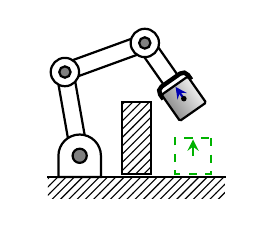
\begin{tikzpicture}
        % Definition of styles
        % function to compute angle and length between coordinates
\makeatletter
\newcommand{\getLengthAndAngle}[2]{%
    \pgfmathanglebetweenpoints{\pgfpointanchor{#1}{center}}
                              {\pgfpointanchor{#2}{center}}
    \global\let\myangle\pgfmathresult % we need a global macro
    \pgfpointdiff{\pgfpointanchor{#1}{center}}
                 {\pgfpointanchor{#2}{center}}
    \pgf@xa=\pgf@x % no need to use a new dimen
    \pgf@ya=\pgf@y
    \pgfmathparse{veclen(\pgf@xa,\pgf@ya)/28.45274} % to convert from pt to cm
    \global\let\mylength\pgfmathresult % we need a global macro
}
\makeatother 
\tikzset{
    pics/pivot/.style args={#1,#2,#3}{
		code = {
			% #1: radius of small circle (pin);
			% #2: radius of large circle (outer dimension).
            % #3: rotation angle
			\draw[thick, fill=white, rotate=#3] (#2,-#2) -- (#2,0) arc(0:180:#2) -- (-#2,-#2) -- cycle;
			\draw[thick, fill=gray] (0,0) circle circle (#1);
		}
	},
	ground/.style = {fill,pattern=north east lines,draw=none,minimum width=1cm,minimum height=1cm},
    spring/.style = {thick,decorate,decoration={zigzag,pre length=4pt,post length=4pt,segment length=3pt}},
    damper/.style = {thick, decoration={markings, mark connection node=dmp, mark=at position 0.5 with
              {
                \node (dmp) [thick,inner sep=0pt,transform shape,rotate=-90,minimum width=8pt,minimum height=2pt,draw=none] {};
                \draw [thick] ($(dmp.north east)+(2pt,0)$) -- (dmp.south east) -- (dmp.south west) -- ($(dmp.north west)+(2pt,0)$);
                \draw [thick] ($(dmp.north)+(0,-3pt)$) -- ($(dmp.north)+(0,3pt)$);
              }
        }, decorate},
	pics/dimLinear/.style args={#1,#2,#3,#4,#5,#6,#7}{
		code = {
			% #1: node 1
			% #2: node 2
			% #3: node 1 guide line distance
			% #4: node 2 guide line distance
			% #5: label distance
			% #6: label
			% #7: label position (ex: right, left, above, below)
			\draw[very thin, gray] ($(#1)!#3!-90:(#2)$) -- ($(#1)!#5+3pt!-90:(#2)$); % lateral line perpendicular to nodes 1 and 2
			\draw[very thin, gray] ($(#2)!#4!90:(#1)$) -- ($(#2)!#5+3pt!90:(#1)$); % lateral line perpendicular to nodes 1 and 2
			\draw[very thin, arrows=<->, gray] ($(#1)!#5!-90:(#2)$) -- ($(#2)!#5!90:(#1)$) node[midway, #7] {#6}; % dimension line parallel to nodes 1 and 2
		}
	},
	pics/dimAngular/.style args={#1,#2,#3,#4,#5,#6,#7,#8}{
		code = {
			% #1: node 1 (this node will define the distance the arc from the central node)
			% #2: node 2
			% #3: node centre
			% #4: distance before arrow ends
			% #5: node 1 guide line distance
			% #6: label
			% #7: label position (ex: right, left, above, below)
			% Create lines for computing arc centre
			\def\argone{#4}\def\argtwo{0}
			\ifx\argone\argtwo % if the arrow offset is zero the rotation centre remains the same
				\coordinate (centre) at (#3);
			\else % if there is offset we find the:
				\draw[name path=AB,draw=none] ($(#2)!#4!90:(#3)$) -- ($(#3)!#4!-90:(#2)$); % line parallel to the link formed by the nodes 1 and 2 with offset #4
				\draw[name path=CD,draw=none] (#1) -- (#3); % reference line for measure the angle
				\coordinate [name intersections={of={AB and CD}}]; % intersection between the offset line and the reference line
				\coordinate (centre) at (intersection-1); % set the rotation centre as the found intersection
			\fi
			\draw [very thin, gray, #8] let
				\p0 = ($(#1)-(centre)$), % difference vector between reference and centre
				\p1 = ($($(#2)!#4!90:(#3)$)-(centre)$) % difference vector reference between the offset line and the centre
				in (#1) arc [start angle={atan2(\y0,\x0)}, end angle={atan2(\y1,\x1)}, radius=({veclen(\y0,\x0)})] node[midway, #7] {#6}; % angular dimension line
			\draw[very thin, gray] ($(#3)!#5!0:(#1)$) -- ($(#1)!-3pt!0:(#3)$); % Draw guide line
		}
	},
    pics/link/.style args={#1,#2,#3}{
		code = {
			% #1: node 1
			% #2: node 2
			% #3: characteristic dimension of drawing
            \draw[thick, fill=white] ($(#1)!1.5*#3!-90:(#2)$) -- ($(#2)!1.5*#3!90:(#1)$) -- ($(#2)!1.5*#3!-90:(#1)$) -- ($(#1)!1.5*#3!90:(#2)$) -- cycle; % lines parallel to nodes 1 and 2
            \fill[white, draw=none] (#2) circle circle (2.5*#3); % outer round part
            \draw[thick] (#2) circle circle (2.5*#3); % outer round part
            \fill[gray, draw=none] (#2) circle circle (#3);
            \draw[thick] (#2) circle circle (#3);
		}
	},
	pics/centreofmass/.style args={#1,#2}{
		code = {
			% #1: radius of symbol
			\draw[fill=black, thin] (#2) -- ++(#1,0) arc [radius=#1, start angle=0,end angle=90] -- ++(0,-2*#1) arc [radius=#1, start angle=270, end angle=180] -- cycle;
			\draw[thin] (#2) circle circle (#1);
		}
	},
	pics/lastlink/.style args={#1,#2,#3}{
		code = {
			% #1: node 1
			% #2: node 2
			% #3: characteristic dimension of drawing
            \coordinate (new2) at ($(#2)!2.0*#3!0:(#1)$);
			\draw[thick] ($(#1)!1.5*#3!-90:(new2)$) -- ($(new2)!1.5*#3!90:(#1)$);
			\draw[thick] ($(#1)!1.5*#3!90:(new2)$) -- ($(new2)!1.5*#3!-90:(#1)$);
			% End-effentor
			\draw[ultra thick,rounded corners=#3] ($($(new2)!2*#3!180:(#1)$)!3*#3!-90:(#1)$) -- ($(new2)!3*#3!-90:(#1)$) -- (new2) -- ($(new2)!3*#3!90:(#1)$) -- ($($(new2)!2*#3!180:(#1)$)!3*#3!90:(#1)$);
		}
	},
    pics/foot/.style args={#1,#2,#3}{
		code = {
			% #1: node 1
			% #2: node 2
			% #3: characteristic dimension of drawing
            \draw[fill=white, very thick, rounded corners=#3] ($(#1)!5.0*#3!-90:(#2)$) -- ($(#2)!1.5*#3!90:(#1)$) -- ($(#2)!1.5*#3!-90:(#1)$) -- ($(#1)!5.0*#3!90:(#2)$) -- cycle;
			%\draw[thick]  -- ;
			% End-effentor
			%\draw[ultra thick,rounded corners=#3] ($($(#2)!2*#3!180:(#1)$)!3*#3!-90:(#1)$) -- ($(#2)!3*#3!-90:(#1)$) -- (#2) -- ($(#2)!3*#3!90:(#1)$) -- ($($(#2)!2*#3!180:(#1)$)!3*#3!90:(#1)$);
            \fill[white, draw=none] (#2) circle circle (2.5*#3); % outer round part
            \draw[thick] (#2) circle circle (2.5*#3); % outer round part
            \fill[gray, draw=none] (#2) circle circle (#3);
            \draw[thick] (#2) circle circle (#3);
		}
	},
    pics/lastlinkcontact/.style args={#1,#2,#3}{
		code = {
			% #1: node 1
			% #2: node 2
			% #3: characteristic dimension of drawing
            % coordinates
            \coordinate (bottomLeft) at ($(#1)!1.5*#3!-90:(#2)$);
            \coordinate (bottomRight) at ($(#2)!1.5*#3!90:(#1)$);
            \coordinate (topLeft) at ($(#1)!1.5*#3!90:(#2)$);
            \coordinate (topRight) at ($(#2)!1.5*#3!-90:(#1)$);
            \coordinate (bottomRight2) at ($(bottomRight)!5.0*#3!0:(bottomLeft)$);
            \coordinate (topRight2) at ($(topRight)!5.0*#3!0:(topLeft)$);
            \coordinate (bottomRight3) at ($(bottomRight)!2.5*#3!0:(bottomLeft)$);
            \coordinate (topRight3) at ($(topRight)!2.5*#3!0:(topLeft)$);
            \pgfmathanglebetweenpoints{\pgfpointanchor{#1}{center}}{\pgfpointanchor{#2}{center}}
            \edef\angle{\pgfmathresult}
            % drawing
            \draw[thick, fill=white] (topLeft) -- (bottomLeft) -- ($(bottomRight2)!0.7!(bottomRight3)$) -- ($(topRight2)!0.7!(topRight3)$) -- cycle;
			% End-effentor
            \draw[thick, fill=gray] (topRight2) arc (\angle+90:\angle-90:1.5*#3) {[rounded corners=1.5pt] -- (bottomRight3)} arc (\angle+180:\angle+90:1.5*#3) coordinate (prov) {[rounded corners=1.5pt] arc (\angle+270:\angle+180:1.5*#3)} -- cycle;
            \draw[thick] (prov) -- (#2);
            \fill[black] (#2) circle (0.5pt);
		}
	},
    pics/limb/.style args={#1,#2,#3,#4}{
		code = {
			% #1: point coordinate 1
			% #2: point coordinate 2
			% #3: thickness of ellipse: 0 - line; 1 - circle
			% #4: scale: 1 is no scale
            % compute myangle and mylength:
            \getLengthAndAngle{#1}{#2}
            % compute central coordinate:
            \coordinate (centre) at ($(#1)!0.5!(#2)$);
            % draw limb
            \draw[rotate=\myangle,shift={(centre)}, very thick, fill=white] (0,0) ellipse ({#4*0.5*\mylength} and {#4*#3*0.5*\mylength});
		}
	},
    pics/square/.style args={#1,#2,#3,#4}{%
        code = {%
            % #1: square centre coordinate
            % #2: inclination angle
            % #3: square size length
			% #4: arrow color
            % ------------------------------
            % draw limb
            \shadedraw[shading angle=#2, cm={cos(-#2) ,-sin(-#2) ,sin(-#2) ,cos(-#2) ,(#1)}, thick, rounded corners=0.5pt] ($(#1)+(0.5*#3,0.5*#3)$) rectangle ($(#1)+(-0.5*#3,-0.5*#3)$);
            \draw[-stealth, #4, thick, cm={cos(-#2) ,-sin(-#2) ,sin(-#2) ,cos(-#2) ,(#1)}] (#1) --++ (0.45*#3,0);
            \fill[black] (#1) circle (1.0pt);
        }
    },
    pics/lastlinklinecontact/.style args={#1,#2,#3}{%
        code = {%
            % #1: node 1
            % #2: node 2
            % #3: characteristic dimension of drawing
            % ------------------------------
            % computing angle between nodes
            \pgfmathanglebetweenpoints{\pgfpointanchor{#1}{center}}{\pgfpointanchor{#2}{center}}
            \edef\angle{\pgfmathresult}
            % coordinates
            \coordinate (bottomRight) at ($(#2)!1.5*#3!90:(#1)$);
            \coordinate (bottomLeft) at ($(#1)!1.5*#3!-90:(#2)$);
            \coordinate (topRight) at ($(#2)!1.5*#3!-90:(#1)$);
            \coordinate (topLeft) at ($(#1)!1.5*#3!90:(#2)$);
            \coordinate (bottomMiddle) at ($(bottomRight)!2.0*#3!0:(bottomLeft)$);
            \coordinate (topMiddle) at ($(topRight)!2.0*#3!0:(topLeft)$);
            \coordinate (bottomBase) at ($(bottomRight)!2.0*#3!180:(topRight)$);
            \coordinate (topBase) at ($(topRight)!2.0*#3!180:(bottomRight)$);
            % drawing
            \draw[thick, fill=white] (bottomLeft) -- (bottomMiddle) -- (topMiddle) -- (topLeft) -- cycle;
            % End-effentor
            \draw[thick, fill=gray, rounded corners=0.5pt] (bottomMiddle)  to [out=\angle-90,in=\angle+135] (bottomBase) -- (topBase) to [out=\angle-135,in=\angle+90] (topMiddle) -- cycle;
        }
    },
    pics/linkwithbreak/.style args={#1,#2,#3}{%
        code = {%
            % #1: node 1
            % #2: node 2
            % #3: characteristic dimension of drawing
            \draw[thick, fill=white] ($(#1)!1.5*#3!-90:(#2)$) -- ($(#2)!1.5*#3!90:(#1)$) -- ($(#2)!1.5*#3!-90:(#1)$) -- ($(#1)!1.5*#3!90:(#2)$); % lines parallel to nodes 1 and 2
            \draw[very thin,line cap=round] ($(#1)!1.5*#3!-90:(#2)$) to [out=-135,in=45, thin] ($(#1)!1.5*#3!90:(#2)$);
            \fill[white, draw=none] (#2) circle circle (2.5*#3); % outer round part
            \draw[thick] (#2) circle circle (2.5*#3); % outer round part
            \fill[gray, draw=none] (#2) circle circle (#3);
            \draw[thick] (#2) circle circle (#3);
        }
    },
    pics/conveyercircle/.style args={#1,#2,#3}{%
        code = {%
            % #1: conveyercircle centre coordinate
            % #2: inclination angle
            % #3: conveyercircle size length
            % ------------------------------
            % draw circle
            \draw[black,fill=black] (#1) circle (0.8*#3);
            \draw[fill=gray!10!white] (#1) circle (0.4*#3);
            \draw[fill=gray!10!white, cm={cos(-#2) ,-sin(-#2) ,sin(-#2) ,cos(-#2) ,(#1)}] ($(#1)+(0.6*#3,0)$) circle (1pt);
            \draw[fill=gray!10!white, cm={cos(-#2) ,-sin(-#2) ,sin(-#2) ,cos(-#2) ,(#1)}] ($(#1)+(0,0.6*#3)$) circle (1pt);
            \draw[fill=gray!10!white, cm={cos(-#2) ,-sin(-#2) ,sin(-#2) ,cos(-#2) ,(#1)}] ($(#1)+(-0.6*#3,0)$) circle (1pt);
            \draw[fill=gray!10!white, cm={cos(-#2) ,-sin(-#2) ,sin(-#2) ,cos(-#2) ,(#1)}] ($(#1)+(0,-0.6*#3)$) circle (1pt);
        }
    },
}
        % Constants for scalling
        \def\U{9mm}
        \coordinate (origin) at (0,0);
        %----------------------------------------------------------------------------
        % previous position
        \def\squared{0.45*\U}
        \def\qa{100}
        \def\qb{-80}
        \def\qc{-75}
        \pgfmathtruncatemacro\qabc{\qa+\qb+\qc+180}
        \coordinate (origin1) at ($(origin)+(\qa:1.2*\U)$);
        \coordinate (origin2) at ($(origin1)!1.2*\U!\qb+180:(origin)$);
        \coordinate (endeffector) at ($(origin2)!0.8*\U!\qc+180:(origin1)$);
        \pic {lastlink={origin2,endeffector,0.08*\U}};
        \pic {link={origin1,origin2,0.08*\U}};
        \pic {link={origin,origin1,0.08*\U}} node[] (link1) {};
        % draw current box
        \coordinate (boxcurrent) at ($(origin2)!1.2!(endeffector)$);
        \pic {square={boxcurrent,\qabc,\squared,black!30!blue}};
        % draw target
        \coordinate (boxtarget) at (1.6*\U,0.0);
        \draw[black!30!green, dashed, thick] ($(boxtarget)+(0.56*\squared,0.56*\squared)$) rectangle ($(boxtarget)+(-0.56*\squared,-0.56*\squared)$);
        \draw[-stealth, black!30!green, thick] (boxtarget) --++ (0,0.23*\U);
        % Draw ground
        \node (ground) at (origin) [ground,yshift=-0.3*\U,anchor=north, minimum width=2.5*\U, xshift=0.8*\U, minimum height=0.3*\U] {};
        \draw[thick] (ground.north east) -- (ground.north west) node[left] {}; % draw ground line
        % draw obstacle
        \node (obstacle) at (0.8*\U,0.0) [ground, yshift=-0.26*\U, anchor=south, minimum width=0.4*\U, minimum height=1.0*\U] {};
        \draw[thick] (obstacle.north east) -- (obstacle.north west) -- (obstacle.south west) -- (obstacle.south east) -- cycle;
        % Draw rotation pivot
        \pic[anchor=north] (pivot) at (origin) {pivot={0.1*\U,0.3*\U,0}};
    \end{tikzpicture}%
    \tikzexternalenable
}%

% figure dual arm
\newsavebox{\nodeDualArm}%
\savebox{\nodeDualArm}{%
    \tikzexternaldisable
    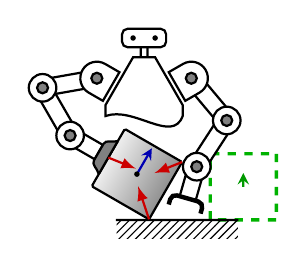
\begin{tikzpicture}[font=\tiny]%
        % Definition of styles
        % function to compute angle and length between coordinates
\makeatletter
\newcommand{\getLengthAndAngle}[2]{%
    \pgfmathanglebetweenpoints{\pgfpointanchor{#1}{center}}
                              {\pgfpointanchor{#2}{center}}
    \global\let\myangle\pgfmathresult % we need a global macro
    \pgfpointdiff{\pgfpointanchor{#1}{center}}
                 {\pgfpointanchor{#2}{center}}
    \pgf@xa=\pgf@x % no need to use a new dimen
    \pgf@ya=\pgf@y
    \pgfmathparse{veclen(\pgf@xa,\pgf@ya)/28.45274} % to convert from pt to cm
    \global\let\mylength\pgfmathresult % we need a global macro
}
\makeatother 
\tikzset{
    pics/pivot/.style args={#1,#2,#3}{
		code = {
			% #1: radius of small circle (pin);
			% #2: radius of large circle (outer dimension).
            % #3: rotation angle
			\draw[thick, fill=white, rotate=#3] (#2,-#2) -- (#2,0) arc(0:180:#2) -- (-#2,-#2) -- cycle;
			\draw[thick, fill=gray] (0,0) circle circle (#1);
		}
	},
	ground/.style = {fill,pattern=north east lines,draw=none,minimum width=1cm,minimum height=1cm},
    spring/.style = {thick,decorate,decoration={zigzag,pre length=4pt,post length=4pt,segment length=3pt}},
    damper/.style = {thick, decoration={markings, mark connection node=dmp, mark=at position 0.5 with
              {
                \node (dmp) [thick,inner sep=0pt,transform shape,rotate=-90,minimum width=8pt,minimum height=2pt,draw=none] {};
                \draw [thick] ($(dmp.north east)+(2pt,0)$) -- (dmp.south east) -- (dmp.south west) -- ($(dmp.north west)+(2pt,0)$);
                \draw [thick] ($(dmp.north)+(0,-3pt)$) -- ($(dmp.north)+(0,3pt)$);
              }
        }, decorate},
	pics/dimLinear/.style args={#1,#2,#3,#4,#5,#6,#7}{
		code = {
			% #1: node 1
			% #2: node 2
			% #3: node 1 guide line distance
			% #4: node 2 guide line distance
			% #5: label distance
			% #6: label
			% #7: label position (ex: right, left, above, below)
			\draw[very thin, gray] ($(#1)!#3!-90:(#2)$) -- ($(#1)!#5+3pt!-90:(#2)$); % lateral line perpendicular to nodes 1 and 2
			\draw[very thin, gray] ($(#2)!#4!90:(#1)$) -- ($(#2)!#5+3pt!90:(#1)$); % lateral line perpendicular to nodes 1 and 2
			\draw[very thin, arrows=<->, gray] ($(#1)!#5!-90:(#2)$) -- ($(#2)!#5!90:(#1)$) node[midway, #7] {#6}; % dimension line parallel to nodes 1 and 2
		}
	},
	pics/dimAngular/.style args={#1,#2,#3,#4,#5,#6,#7,#8}{
		code = {
			% #1: node 1 (this node will define the distance the arc from the central node)
			% #2: node 2
			% #3: node centre
			% #4: distance before arrow ends
			% #5: node 1 guide line distance
			% #6: label
			% #7: label position (ex: right, left, above, below)
			% Create lines for computing arc centre
			\def\argone{#4}\def\argtwo{0}
			\ifx\argone\argtwo % if the arrow offset is zero the rotation centre remains the same
				\coordinate (centre) at (#3);
			\else % if there is offset we find the:
				\draw[name path=AB,draw=none] ($(#2)!#4!90:(#3)$) -- ($(#3)!#4!-90:(#2)$); % line parallel to the link formed by the nodes 1 and 2 with offset #4
				\draw[name path=CD,draw=none] (#1) -- (#3); % reference line for measure the angle
				\coordinate [name intersections={of={AB and CD}}]; % intersection between the offset line and the reference line
				\coordinate (centre) at (intersection-1); % set the rotation centre as the found intersection
			\fi
			\draw [very thin, gray, #8] let
				\p0 = ($(#1)-(centre)$), % difference vector between reference and centre
				\p1 = ($($(#2)!#4!90:(#3)$)-(centre)$) % difference vector reference between the offset line and the centre
				in (#1) arc [start angle={atan2(\y0,\x0)}, end angle={atan2(\y1,\x1)}, radius=({veclen(\y0,\x0)})] node[midway, #7] {#6}; % angular dimension line
			\draw[very thin, gray] ($(#3)!#5!0:(#1)$) -- ($(#1)!-3pt!0:(#3)$); % Draw guide line
		}
	},
    pics/link/.style args={#1,#2,#3}{
		code = {
			% #1: node 1
			% #2: node 2
			% #3: characteristic dimension of drawing
            \draw[thick, fill=white] ($(#1)!1.5*#3!-90:(#2)$) -- ($(#2)!1.5*#3!90:(#1)$) -- ($(#2)!1.5*#3!-90:(#1)$) -- ($(#1)!1.5*#3!90:(#2)$) -- cycle; % lines parallel to nodes 1 and 2
            \fill[white, draw=none] (#2) circle circle (2.5*#3); % outer round part
            \draw[thick] (#2) circle circle (2.5*#3); % outer round part
            \fill[gray, draw=none] (#2) circle circle (#3);
            \draw[thick] (#2) circle circle (#3);
		}
	},
	pics/centreofmass/.style args={#1,#2}{
		code = {
			% #1: radius of symbol
			\draw[fill=black, thin] (#2) -- ++(#1,0) arc [radius=#1, start angle=0,end angle=90] -- ++(0,-2*#1) arc [radius=#1, start angle=270, end angle=180] -- cycle;
			\draw[thin] (#2) circle circle (#1);
		}
	},
	pics/lastlink/.style args={#1,#2,#3}{
		code = {
			% #1: node 1
			% #2: node 2
			% #3: characteristic dimension of drawing
            \coordinate (new2) at ($(#2)!2.0*#3!0:(#1)$);
			\draw[thick] ($(#1)!1.5*#3!-90:(new2)$) -- ($(new2)!1.5*#3!90:(#1)$);
			\draw[thick] ($(#1)!1.5*#3!90:(new2)$) -- ($(new2)!1.5*#3!-90:(#1)$);
			% End-effentor
			\draw[ultra thick,rounded corners=#3] ($($(new2)!2*#3!180:(#1)$)!3*#3!-90:(#1)$) -- ($(new2)!3*#3!-90:(#1)$) -- (new2) -- ($(new2)!3*#3!90:(#1)$) -- ($($(new2)!2*#3!180:(#1)$)!3*#3!90:(#1)$);
		}
	},
    pics/foot/.style args={#1,#2,#3}{
		code = {
			% #1: node 1
			% #2: node 2
			% #3: characteristic dimension of drawing
            \draw[fill=white, very thick, rounded corners=#3] ($(#1)!5.0*#3!-90:(#2)$) -- ($(#2)!1.5*#3!90:(#1)$) -- ($(#2)!1.5*#3!-90:(#1)$) -- ($(#1)!5.0*#3!90:(#2)$) -- cycle;
			%\draw[thick]  -- ;
			% End-effentor
			%\draw[ultra thick,rounded corners=#3] ($($(#2)!2*#3!180:(#1)$)!3*#3!-90:(#1)$) -- ($(#2)!3*#3!-90:(#1)$) -- (#2) -- ($(#2)!3*#3!90:(#1)$) -- ($($(#2)!2*#3!180:(#1)$)!3*#3!90:(#1)$);
            \fill[white, draw=none] (#2) circle circle (2.5*#3); % outer round part
            \draw[thick] (#2) circle circle (2.5*#3); % outer round part
            \fill[gray, draw=none] (#2) circle circle (#3);
            \draw[thick] (#2) circle circle (#3);
		}
	},
    pics/lastlinkcontact/.style args={#1,#2,#3}{
		code = {
			% #1: node 1
			% #2: node 2
			% #3: characteristic dimension of drawing
            % coordinates
            \coordinate (bottomLeft) at ($(#1)!1.5*#3!-90:(#2)$);
            \coordinate (bottomRight) at ($(#2)!1.5*#3!90:(#1)$);
            \coordinate (topLeft) at ($(#1)!1.5*#3!90:(#2)$);
            \coordinate (topRight) at ($(#2)!1.5*#3!-90:(#1)$);
            \coordinate (bottomRight2) at ($(bottomRight)!5.0*#3!0:(bottomLeft)$);
            \coordinate (topRight2) at ($(topRight)!5.0*#3!0:(topLeft)$);
            \coordinate (bottomRight3) at ($(bottomRight)!2.5*#3!0:(bottomLeft)$);
            \coordinate (topRight3) at ($(topRight)!2.5*#3!0:(topLeft)$);
            \pgfmathanglebetweenpoints{\pgfpointanchor{#1}{center}}{\pgfpointanchor{#2}{center}}
            \edef\angle{\pgfmathresult}
            % drawing
            \draw[thick, fill=white] (topLeft) -- (bottomLeft) -- ($(bottomRight2)!0.7!(bottomRight3)$) -- ($(topRight2)!0.7!(topRight3)$) -- cycle;
			% End-effentor
            \draw[thick, fill=gray] (topRight2) arc (\angle+90:\angle-90:1.5*#3) {[rounded corners=1.5pt] -- (bottomRight3)} arc (\angle+180:\angle+90:1.5*#3) coordinate (prov) {[rounded corners=1.5pt] arc (\angle+270:\angle+180:1.5*#3)} -- cycle;
            \draw[thick] (prov) -- (#2);
            \fill[black] (#2) circle (0.5pt);
		}
	},
    pics/limb/.style args={#1,#2,#3,#4}{
		code = {
			% #1: point coordinate 1
			% #2: point coordinate 2
			% #3: thickness of ellipse: 0 - line; 1 - circle
			% #4: scale: 1 is no scale
            % compute myangle and mylength:
            \getLengthAndAngle{#1}{#2}
            % compute central coordinate:
            \coordinate (centre) at ($(#1)!0.5!(#2)$);
            % draw limb
            \draw[rotate=\myangle,shift={(centre)}, very thick, fill=white] (0,0) ellipse ({#4*0.5*\mylength} and {#4*#3*0.5*\mylength});
		}
	},
    pics/square/.style args={#1,#2,#3,#4}{%
        code = {%
            % #1: square centre coordinate
            % #2: inclination angle
            % #3: square size length
			% #4: arrow color
            % ------------------------------
            % draw limb
            \shadedraw[shading angle=#2, cm={cos(-#2) ,-sin(-#2) ,sin(-#2) ,cos(-#2) ,(#1)}, thick, rounded corners=0.5pt] ($(#1)+(0.5*#3,0.5*#3)$) rectangle ($(#1)+(-0.5*#3,-0.5*#3)$);
            \draw[-stealth, #4, thick, cm={cos(-#2) ,-sin(-#2) ,sin(-#2) ,cos(-#2) ,(#1)}] (#1) --++ (0.45*#3,0);
            \fill[black] (#1) circle (1.0pt);
        }
    },
    pics/lastlinklinecontact/.style args={#1,#2,#3}{%
        code = {%
            % #1: node 1
            % #2: node 2
            % #3: characteristic dimension of drawing
            % ------------------------------
            % computing angle between nodes
            \pgfmathanglebetweenpoints{\pgfpointanchor{#1}{center}}{\pgfpointanchor{#2}{center}}
            \edef\angle{\pgfmathresult}
            % coordinates
            \coordinate (bottomRight) at ($(#2)!1.5*#3!90:(#1)$);
            \coordinate (bottomLeft) at ($(#1)!1.5*#3!-90:(#2)$);
            \coordinate (topRight) at ($(#2)!1.5*#3!-90:(#1)$);
            \coordinate (topLeft) at ($(#1)!1.5*#3!90:(#2)$);
            \coordinate (bottomMiddle) at ($(bottomRight)!2.0*#3!0:(bottomLeft)$);
            \coordinate (topMiddle) at ($(topRight)!2.0*#3!0:(topLeft)$);
            \coordinate (bottomBase) at ($(bottomRight)!2.0*#3!180:(topRight)$);
            \coordinate (topBase) at ($(topRight)!2.0*#3!180:(bottomRight)$);
            % drawing
            \draw[thick, fill=white] (bottomLeft) -- (bottomMiddle) -- (topMiddle) -- (topLeft) -- cycle;
            % End-effentor
            \draw[thick, fill=gray, rounded corners=0.5pt] (bottomMiddle)  to [out=\angle-90,in=\angle+135] (bottomBase) -- (topBase) to [out=\angle-135,in=\angle+90] (topMiddle) -- cycle;
        }
    },
    pics/linkwithbreak/.style args={#1,#2,#3}{%
        code = {%
            % #1: node 1
            % #2: node 2
            % #3: characteristic dimension of drawing
            \draw[thick, fill=white] ($(#1)!1.5*#3!-90:(#2)$) -- ($(#2)!1.5*#3!90:(#1)$) -- ($(#2)!1.5*#3!-90:(#1)$) -- ($(#1)!1.5*#3!90:(#2)$); % lines parallel to nodes 1 and 2
            \draw[very thin,line cap=round] ($(#1)!1.5*#3!-90:(#2)$) to [out=-135,in=45, thin] ($(#1)!1.5*#3!90:(#2)$);
            \fill[white, draw=none] (#2) circle circle (2.5*#3); % outer round part
            \draw[thick] (#2) circle circle (2.5*#3); % outer round part
            \fill[gray, draw=none] (#2) circle circle (#3);
            \draw[thick] (#2) circle circle (#3);
        }
    },
    pics/conveyercircle/.style args={#1,#2,#3}{%
        code = {%
            % #1: conveyercircle centre coordinate
            % #2: inclination angle
            % #3: conveyercircle size length
            % ------------------------------
            % draw circle
            \draw[black,fill=black] (#1) circle (0.8*#3);
            \draw[fill=gray!10!white] (#1) circle (0.4*#3);
            \draw[fill=gray!10!white, cm={cos(-#2) ,-sin(-#2) ,sin(-#2) ,cos(-#2) ,(#1)}] ($(#1)+(0.6*#3,0)$) circle (1pt);
            \draw[fill=gray!10!white, cm={cos(-#2) ,-sin(-#2) ,sin(-#2) ,cos(-#2) ,(#1)}] ($(#1)+(0,0.6*#3)$) circle (1pt);
            \draw[fill=gray!10!white, cm={cos(-#2) ,-sin(-#2) ,sin(-#2) ,cos(-#2) ,(#1)}] ($(#1)+(-0.6*#3,0)$) circle (1pt);
            \draw[fill=gray!10!white, cm={cos(-#2) ,-sin(-#2) ,sin(-#2) ,cos(-#2) ,(#1)}] ($(#1)+(0,-0.6*#3)$) circle (1pt);
        }
    },
}
        % Constants for scalling
        \def\U{7.0mm}
        \coordinate (origin) at (0,0);
        \coordinate (shoulderL) at (-0.6,2.27*\U);
        \coordinate (shoulderR) at (0.6,2.27*\U);
        %----------------------------------------------------------------------------
        % previous position
        \def\squared{1.2*\U}
        \def\qLbase{60}
        \def\qLshoulder{-170.0}
        \def\qLelbow{110.0}
        \def\qLwrist{30.0}
        \def\qRbase{-60}
        \def\qRshoulder{-50.0}
        \def\qRelbow{-73.0}
        \def\qRwrist{17.0}
        \pgfmathparse{\qLshoulder+\qLelbow+\qLwrist}
        \edef\qL{\pgfmathresult}
        % left arm coordinates
        \coordinate (elbowL) at ($(shoulderL)+(\qLshoulder:1.0*\U)$);
        \coordinate (wristL) at ($(elbowL)!1.0*\U!180+\qLelbow:(shoulderL)$);
        \coordinate (endeffectorL) at ($(wristL)!0.8*\U!180+\qLwrist:(elbowL)$);
        % right arm coordinates
        \coordinate (elbowR) at ($(shoulderR)+(\qRshoulder:1.0*\U)$);
        \coordinate (wristR) at ($(elbowR)!1.0*\U!180+\qRelbow:(shoulderR)$);
        \coordinate (endeffectorR) at ($(wristR)!0.8*\U!180+\qRwrist:(elbowR)$);
        % box coordinates
        \coordinate (boxcurrent) at ($(endeffectorL)!0.5*\squared!180:(wristL)$);
        \coordinate (boxtarget) at (1.8*\U,0.3*\U);
        \begin{scope}[transparency group]
            % draw box target
            \draw[black!30!green, dashed, very thick] ($(boxtarget)+(0.5*\squared,0.5*\squared)$) rectangle ($(boxtarget)+(-0.5*\squared,-0.5*\squared)$);
            \draw[-stealth, mygreen, thick] (boxtarget) --++ (0,0.25*\U);
            % draw neck
            \draw[thick, fill=white] (-0.06*\U,2.6*\U) rectangle (0.06*\U,2.9*\U);
            % draw body
            \draw[thick, fill=white] (0,2.65*\U) -- ++(0.2*\U,0) -- ++(\qRbase:1.0*\U) -- ++(0,-0.2*\U) to[in=20,out=-110] ++(-1.4*\U,0) -- ++(0,0.2*\U) -- ++(\qLbase:1.0*\U) -- cycle;
            % draw head
            \node [draw, fill=white, thick, shape=rectangle, minimum width=0.8*\U, minimum height=0.2*\U, anchor=center, rounded corners=2pt] at (0,3.0*\U) {};
            \fill[black] (0.2*\U,3.0*\U) circle (1.0pt) node[] {};
            \fill[black] (-0.2*\U,3.0*\U) circle (1.0pt) node[] {};
            % draw box current 
            \pic {square={boxcurrent,\qL-90,\squared,black!30!blue}};
            % draw left arm
            \pic {lastlinklinecontact={wristL,endeffectorL,0.1*\U}};
            \pic {link={elbowL,wristL,0.1*\U}};
            \pic {link={shoulderL,elbowL,0.1*\U}} node[] (link1) {};
            \pic[anchor=north] (pivot) at (shoulderL) {pivot={0.1*\U,0.3*\U,\qLbase}};
            % draw right arm
            \pic {lastlink={wristR,endeffectorR,0.1*\U}};
            \pic {link={elbowR,wristR,0.1*\U}};
            \pic {link={shoulderR,elbowR,0.1*\U}} node[] (link1) {};
            \pic[anchor=north] (pivot) at (shoulderR) {pivot={0.1*\U,0.3*\U,\qRbase}};
            % \fill[black] (endeffectorR) circle (1.0pt) node[] {};
            % Draw ground
            \node (ground) at (origin) [ground,yshift=-0.3*\U,anchor=north, minimum width=2.2*\U, xshift=0.6*\U, minimum height=0.3*\U] {};
            \draw[thick] (ground.north east) -- (ground.north west) node[left] {}; % draw ground line
            % draw box motion
            % \draw[-stealth, double, myred, thick] ($(boxcurrent)+(0.5*\U,0.6*\U)$) -- node {} ++(0.6*\U,0);
            % draw forces
            \draw[-latex, myred, thick] (endeffectorL) -- ++(0.5*\U,-0.2*\U) node[] {};
            \coordinate (boxcornerA) at ($(boxcurrent)+(\qL-90:0.5*\squared)+(\qL:0.5*\squared)$);
            \draw[-latex, myred, thick] (boxcornerA) -- ++(-0.2*\U,0.6*\U) node[] {};
            \coordinate (boxcornerB) at ($(boxcurrent)+(\qL+90:0.5*\squared)+(\qL:0.5*\squared)$);
            \draw[-latex, myred, thick] (boxcornerB) -- ++(-0.5*\U,-0.2*\U) node[] {};
        \end{scope}
    \end{tikzpicture}%
    \tikzexternalenable
}%
% remove Figure from figures caption
\setbeamertemplate{caption}{\raggedright\insertcaption\par}

\begin{frame}[plain,noframenumbering]
  \maketitle
\end{frame}

% Outline frame
\begin{frame}{Outline}
    \tableofcontents
\end{frame}

\section{Manipulation Workshop}

\begin{frame}{UK Robot Manipulation Workshop\footnote{\href{https://www.robot-manipulation.uk}{www.robot-manipulation.uk}}}
  \begin{center}
    \begin{figure}
      \fbox{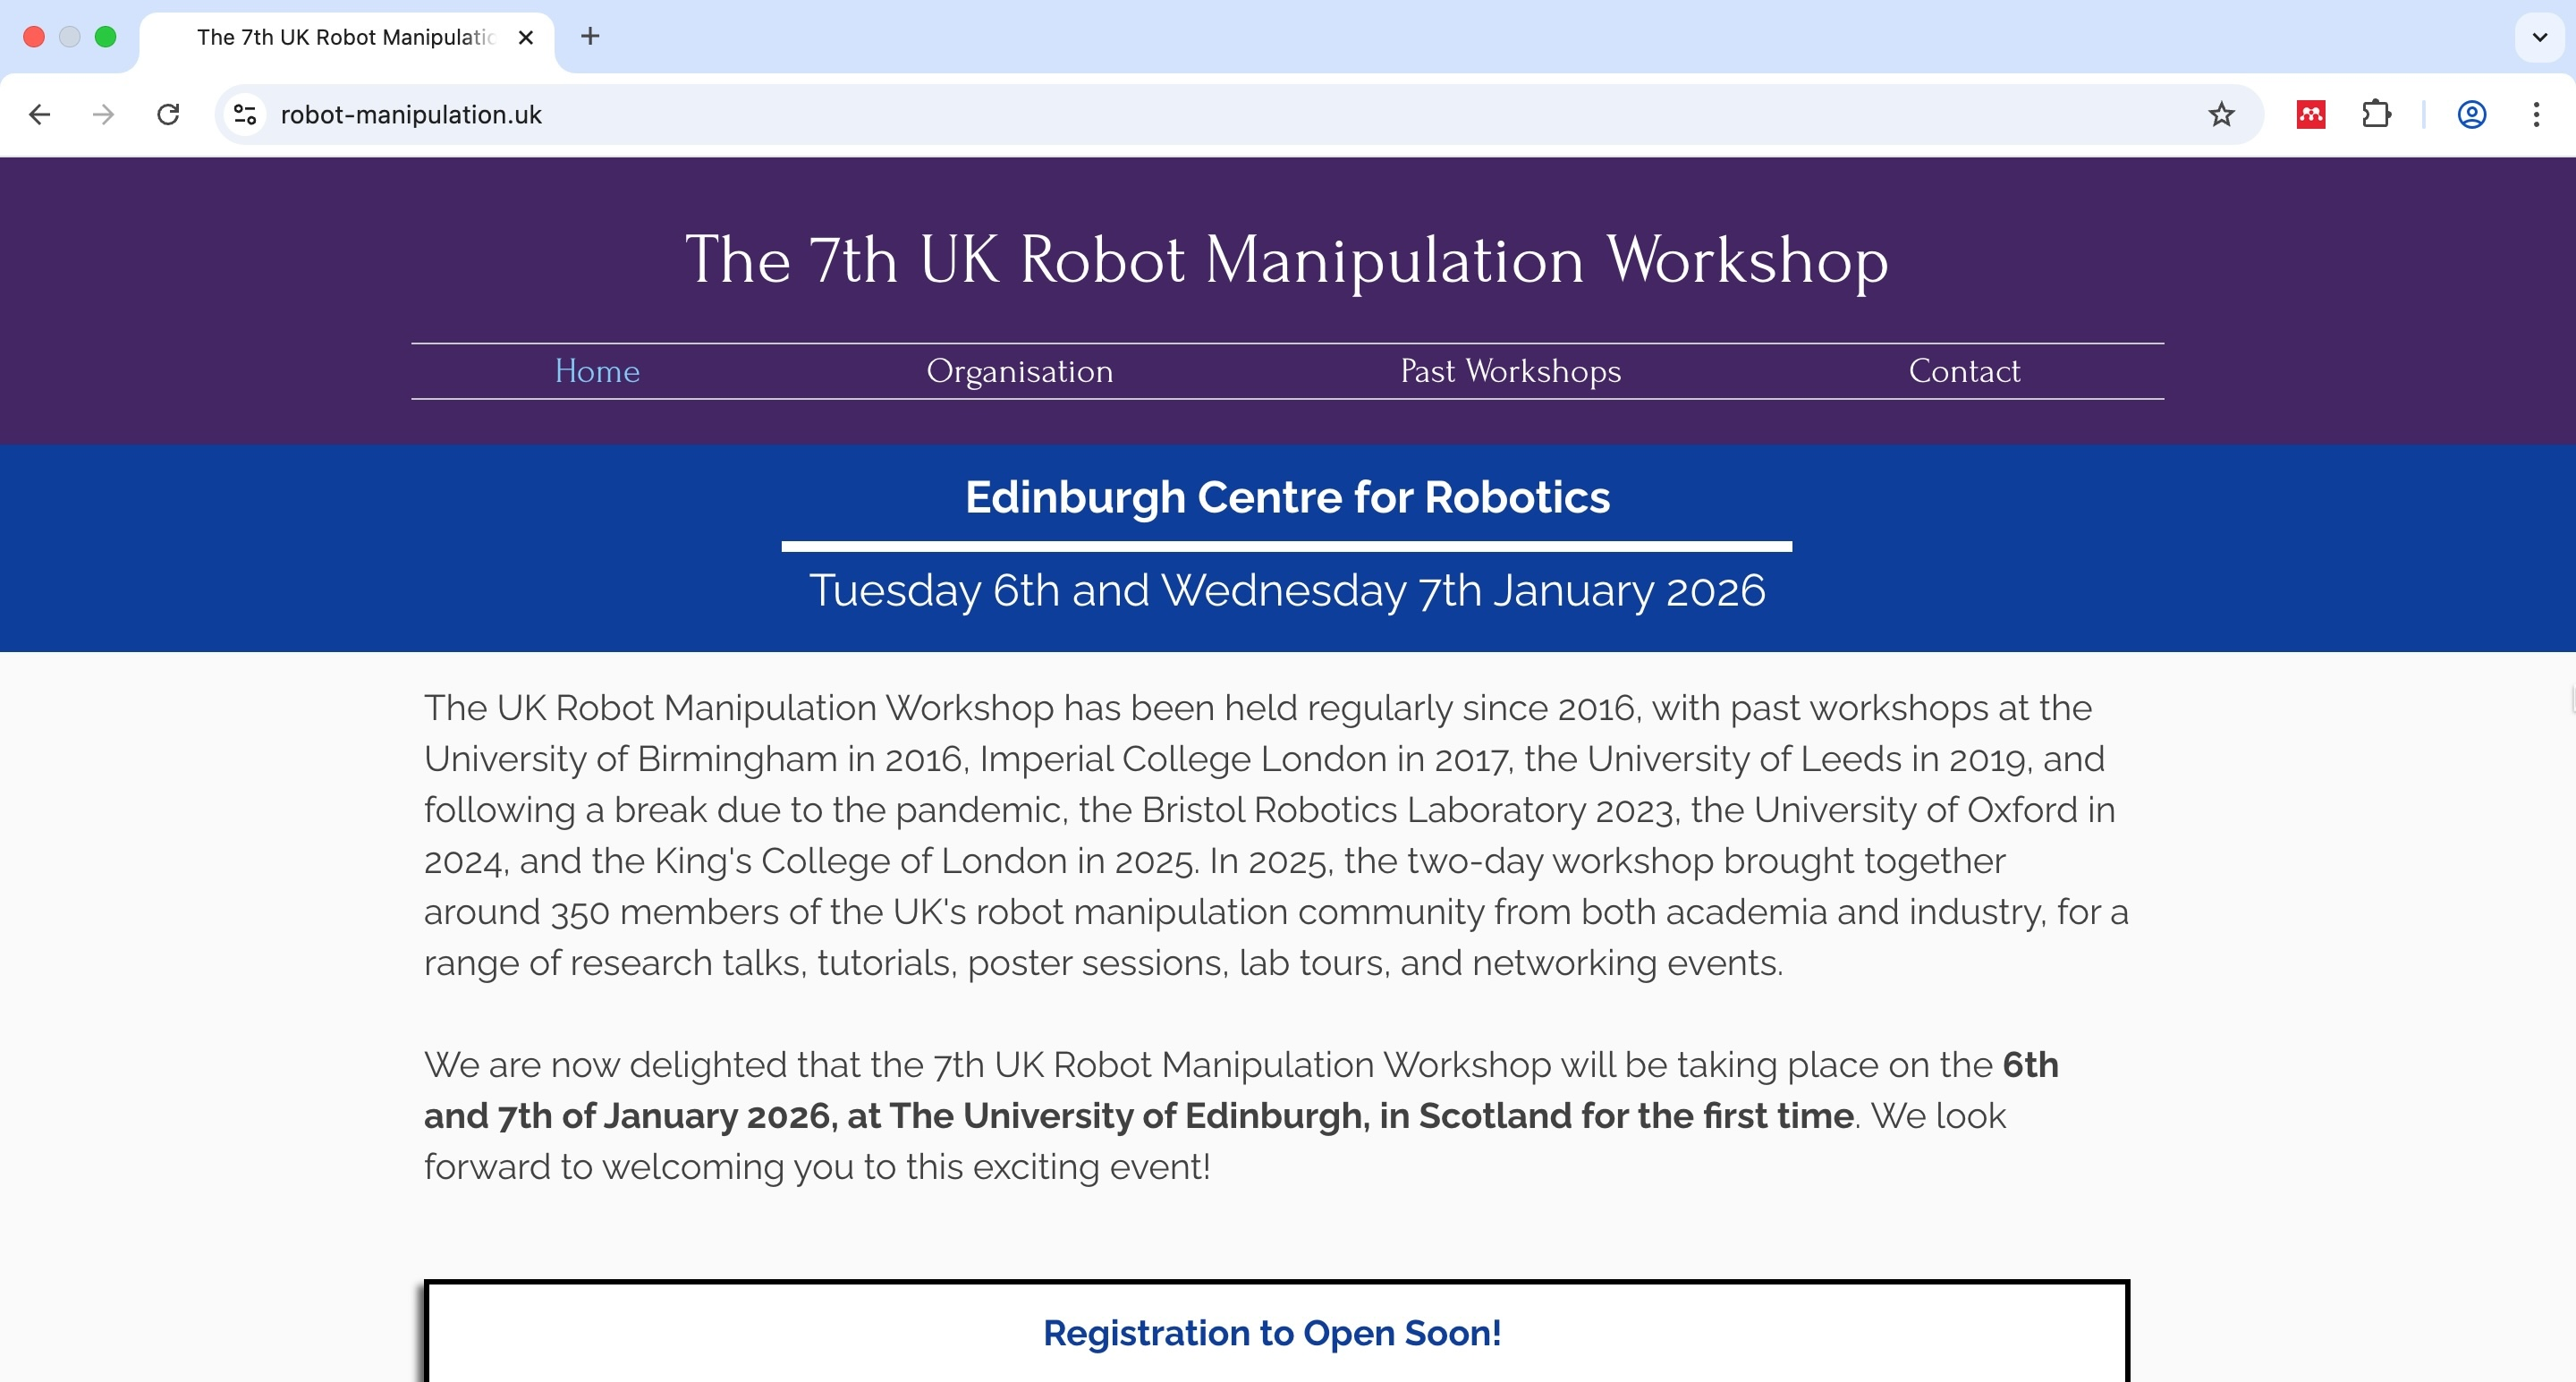
\includegraphics[width=0.8\textwidth]{images/uk_robot_manipulation.jpg}}
    \end{figure}
  \end{center}
\end{frame}

\section{Project applications}

\begin{frame}{
  UKRI applications\footnote{\href{https://www.ukri.org/opportunity/japan-uk-joint-call-for-collaborations-in-advancing-human-centred-ai/}{ukri.org/opportunity/japan-uk-joint-call-for-collaborations-in-advancing-human-centred-ai/}}
  }{Scaling Whole-Body Contact-Rich Interactions for Assistive Robotics: Human Centric Innovations for Embodied AI}
  \begin{center}
    \begin{figure}
      \includegraphics[width=0.7\textwidth]{images/fig_ukri_diagram.pdf}
    \end{figure}
  \end{center}
\end{frame}

\section{Research}

\begin{frame}[plain, noframenumbering]
  \maketitle
\end{frame}

\end{document}
